\documentclass[12pt]{article}
\usepackage{amsmath}
\usepackage{amssymb}
\usepackage{graphicx}
\usepackage{enumitem}
\usepackage{mathtools}
\usepackage{textcomp}
\usepackage[left=2cm,right=2cm,top=2cm,bottom=2cm]{geometry}
\usepackage{rsfso}
\usepackage{listingsutf8}
\usepackage{hyperref}
\usepackage{multicol}
\usepackage{tikz}
\usetikzlibrary{decorations.markings,trees}
\usepackage{forest}
\everymath{\displaystyle}

\lstset{
  language=C,
  inputencoding=utf8,
  extendedchars=true,
  basicstyle=\ttfamily\footnotesize,
  numberstyle=\tiny\color{gray},
  stepnumber=1,
  numbersep=5pt,
  showstringspaces=false,
  breaklines=true,
  tabsize=1,
  literate=
      {ñ}{{\~n}}1
      {Ñ}{{\~N}}1
      {á}{{\'a}}1
      {é}{{\'e}}1
      {í}{{\'i}}1
      {ó}{{\'o}}1
      {ú}{{\'u}}1
      {Á}{{\'A}}1
      {É}{{\'E}}1
      {Í}{{\'Í}}1
      {Ó}{{\'Ó}}1
      {Ú}{{\'Ú}}1
}

\begin{document}

  \begin{titlepage}
      \centering
      
\includegraphics[width=0.3\textwidth]{../imgs/logo-uai-fic.png}

      \vspace{0.5cm}
      \textbf{\fontsize{12}{24} Ayudantía 10: Repaso Árboles y Grafos}

      \vspace{0.5cm}
      \textbf{\fontsize{12}{24}\selectfont Profesores: Sebastián Sáez, Diego Ramos}

      \begin{center}
        \textbf{\fontsize{12}{24}\selectfont Ayudantes: Diego Duhalde, Benjamín Wiedmaier, Fernando Zamora}
      \end{center}

      \begin{center}
        \textbf{PREGUNTAS}
      \end{center}

      \begin{enumerate}[leftmargin=*]
        % EJERCICIO 1
        \item Defina brevemente los siguientes términos en el contexto de árboles binarios:
        \begin{enumerate}[label=\alph*)]
          \item \emph{Grado} de un nodo.
          \item \emph{Descendiente} y \emph{ancestro} de un nodo.
          \item \emph{Camino} en un árbol y \emph{distancia} entre dos nodos.
          \item Diferencia entre un \emph{árbol binario completo} y un \emph{árbol binario perfecto}.
        \end{enumerate}

        % EJERCICIO 2
        \item Dado el siguiente árbol binario de búsqueda:
        \[
        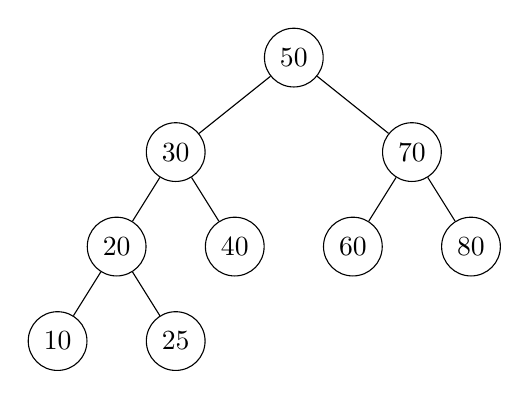
\begin{tikzpicture}[level distance=1.2cm,
          level 1/.style={sibling distance=3cm},
          level 2/.style={sibling distance=1.5cm}]
          \node[circle,draw] (N50) {50}
            child { node[circle,draw] (N30) {30}
              child { node[circle,draw] (N20) {20}
                child { node[circle,draw] (N10) {10} }
                child { node[circle,draw] (N25) {25} }
              }
              child { node[circle,draw] (N40) {40} }
            }
            child { node[circle,draw] (N70) {70}
              child { node[circle,draw] (N60) {60} }
              child { node[circle,draw] (N80) {80} }
            };
        \end{tikzpicture}
        \]
        \begin{enumerate}[label=\alph*)]
          \item Escriba el resultado del recorrido \emph{in-order}.
          \item Escriba el resultado del recorrido \emph{post-order}.
          \item Si eliminamos el nodo con valor 30, muestre el nuevo árbol resultante (dibújelo).
        \end{enumerate}

        % EJERCICIO 3
        \item Inserte en un árbol AVL inicialmente vacío las claves, en orden:
        \[
        40,\; 20,\; 10,\; 30,\; 50,\; 45,\; 60,\; 5.
        \]
        Dibuje el árbol después de cada inserción y anote las alturas de cada nodo. En el caso de que se produzca un desbalance, indique el tipo de rotación que se aplica y dibuje el árbol resultante.
        
        \newpage

        % EJERCICIO 4
        \item Sea el siguiente grafo no dirigido y ponderado con vértices \(\{A,B,C,D,E\}\):

        \begin{center}
          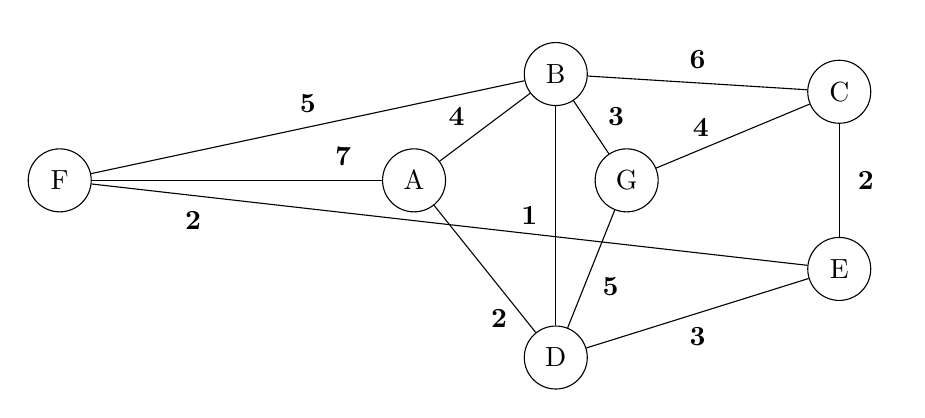
\begin{tikzpicture}[scale=0.9, every node/.style={circle, draw, minimum size=8mm}]
            \node (A) at (0,0) {A};
            \node (B) at (2,1.5) {B};
            \node (C) at (6,1.25) {C};
            \node (D) at (2,-2.5) {D};
            \node (E) at (6,-1.25) {E};
            \node (F) at (-5, 0) {F};
            \node (G) at (3, 0) {G};

            \draw (A) -- (B);
            \node[draw=none, above, font=\bfseries] at ($(A)!0.3!(B)$) {4};
            
            \draw (A) -- (D);
            \node[draw=none, below, font=\bfseries] at ($(A)!0.6!(D)$) {2};

            \draw (A) -- (F);
            \node[draw=none, above, yshift=-0.3em, font=\bfseries] at ($(A)!0.2!(F)$) {7};

            \draw (B) -- (C);
            \node[draw=none, above, yshift=-0.3em, font=\bfseries] at ($(B)!0.5!(C)$) {6};
            
            \draw (B) -- (F);
            \node[draw=none, above, yshift=-0.3em, font=\bfseries] at ($(B)!0.5!(F)$) {5};
            
            \draw (B) -- (G);
            \node[draw=none, right, font=\bfseries] at ($(B)!0.4!(G)$) {3};
            
            \draw (B) -- (D);
            \node[draw=none, left, xshift=0.2em, font=\bfseries] at ($(B)!0.5!(D)$) {1};
            
            \draw (C) -- (E);
            \node[draw=none, right, xshift=-0.2em, font=\bfseries] at ($(C)!0.5!(E)$) {2};
            
            \draw (C) -- (G);
            \node[draw=none, left, yshift=0.3em, font=\bfseries] at ($(C)!0.5!(G)$) {4};
            
            \draw (D) -- (E);
            \node[draw=none, below, yshift=0.3em, font=\bfseries] at ($(D)!0.5!(E)$) {3};
            
            \draw (D) -- (G);
            \node[draw=none, right, xshift=-0.2em, font=\bfseries] at ($(D)!0.4!(G)$) {5};
            
            \draw (E) -- (F);
            \node[draw=none, below left, font=\bfseries] at ($(E)!0.8!(F)$) {2};
          \end{tikzpicture}
        \end{center}

        \begin{enumerate}[label=\alph*)]
          \item Escriba la matriz de adyacencia del grafo.
          \item ¿Es conexo este grafo? ¿Contiene al menos un ciclo? Explique brevemente.
        \end{enumerate}

        % EJERCICIO 5
        \item Para el grafo del ejercicio anterior:
        \begin{enumerate}[label=\alph*)]
          \item Aplique \emph{Kruskal}: indique el orden en que se agregan las aristas y dibuje el árbol resultante con su peso total.
          \item Aplique \emph{Prim} partiendo desde el vértice \(A\): en cada paso anote la arista elegida y el vértice agregado. Termine con el peso total.
          \item ¿Coinciden ambos MSTs? ¿Por qué?
        \end{enumerate}

        % EJERCICIO 6
        \item Considere el grafo del ejercicio 4 y realice lo siguiente:
        \begin{enumerate}[label=\alph*)]
          \item Ejecute paso a paso \emph{Dijkstra} desde \(A\).
          \item Indique el camino más corto de \(A\) a \(E\) y su distancia total.
        \end{enumerate}
    \end{enumerate}
  \end{titlepage}

  \newpage
      \begin{center}
          \textbf{RESPUESTAS}
      \end{center}

      \begin{enumerate}
        % RESPUESTA 1
        \item
          \begin{enumerate}[label=\alph*)]
            \item El grado de un nodo es el número de hijos que tiene.
            \item Un descendiente de un nodo es cualquier nodo que se encuentra en el subárbol cuya raíz es ese nodo. Un ancestro de un nodo es cualquier nodo en el camino desde la raíz hasta ese nodo (incluyendo la raíz, pero excluyendo el propio nodo).
            \item Un camino en un árbol es una secuencia de nodos conectados por aristas consecutivas. La distancia entre dos nodos es el número de aristas en el camino más corto que los conecta.
            \item Un árbol binario completo es aquel en el que todos los niveles, excepto posiblemente el último, están completamente llenos y todos los nodos están lo más a la izquierda posible. Un árbol binario perfecto es aquel en el que todos los niveles están completamente llenos.
          \end{enumerate}

        % RESPUESTA 2
        \item
          \begin{enumerate}[label=\alph*)]
            \item El recorrido in-order es: 10, 20, 25, 30, 40, 50, 60, 70, 80.

            \item El recorrido post-order es: 10, 25, 20, 40, 30, 60, 80, 70, 50.

            \item El árbol resultante tras eliminar el nodo 30 es:

            \[
            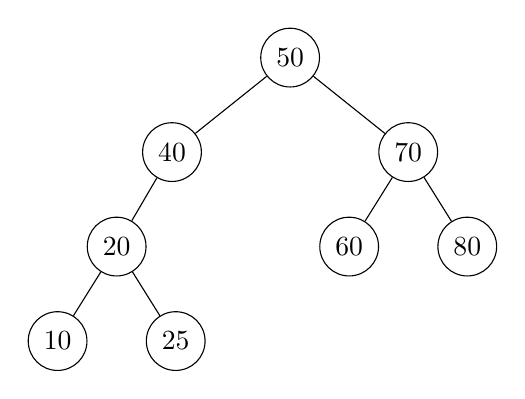
\begin{tikzpicture}[level distance=1.2cm,
              level 1/.style={sibling distance=3cm},
              level 2/.style={sibling distance=1.5cm}]
              \node[circle,draw] (N50) {50}
                child { node[circle,draw] (N40) {40}
                  child { node[circle,draw, xshift=-2em] (N20) {20}
                    child { node[circle,draw] (N10) {10} }
                    child { node[circle,draw] (N25) {25} }
                  }           
                }
                child { node[circle,draw] (N70) {70}
                  child { node[circle,draw] (N60) {60} }
                  child { node[circle,draw] (N80) {80} }
                };
            \end{tikzpicture}
            \]
          \end{enumerate}

        % RESPUESTA 3
        \item Paso a paso de las inserciones y alturas y consideremos que \( bf = h_{subgrafoI} - h_{subgrafoD}\)
          \begin{itemize}
            \item \textbf{Insertar 40}:
            \[
              \begin{forest}
                for tree={circle,draw,minimum size=1.2em,inner sep=1pt,s sep=3em,l=3em}
                [40, label=above:{\textbf{bf: 0}}]
              \end{forest}
            \]
            Altura de 50: 1. No hay rotación.

            \vspace{1em}
            \item \textbf{Insertar 20}:
            \[
              \begin{forest}
                for tree={circle,draw,minimum size=1.2em,inner sep=1pt,s sep=3em,l=3em}
                [40, label=above:{\textbf{bf: 1}}
                  [20, label=above left:{\textbf{bf: 0}}, xshift=-2em]        
                ]
              \end{forest}
            \]
            Alturas: 40 (2), 20 (1). No hay rotación.
            \vspace{1em}

            \item \textbf{Insertar 10}:
            \[
              \begin{forest}
                for tree={circle,draw,minimum size=1.2em,inner sep=1pt,s sep=3em,l=3em}
                [40, label=above:{\textbf{bf: 2}}
                  [20, label=above left:{\textbf{bf: 1}}, xshift=-2em
                    [10, label=above left:{\textbf{bf: 0}}, xshift=-4em]
                  ]
                ]
              \end{forest}
            \]
            Alturas: 40 (3), 20 (2), 10 (1). \\
            \textbf{Rotación:} Hay un desbalance en el nodo 40 (izquierda izquierda), se aplica una rotación simple a la derecha.
            \[
              \begin{forest}
                for tree={circle,draw,minimum size=1.2em,inner sep=1pt,s sep=3em,l=3em}
                [20, label=above:{\textbf{bf: 0}}
                  [10, label=above left:{\textbf{bf: 0}}, xshift=-2em]
                  [40, label=above right:{\textbf{bf: 0}}, xshift=2em]
                ]
              \end{forest}
            \]
            Alturas: 20 (2), 10 (1), 40 (1). No hay más desbalance.
            \vspace{1em}

            \item \textbf{Insertar 30}:
            \[
              \begin{forest}
                for tree={circle,draw,minimum size=1.2em,inner sep=1pt,s sep=3em,l=3em}
                [20, label=above:\textbf{bf: -1}
                  [10, label=above left:{\textbf{bf: 0}}]
                  [40, label=above right:{\textbf{bf: -1}}
                    [30, label=above right:{\textbf{bf: 0}}, xshift=2em]
                  ]
                ]
              \end{forest}
            \]
            Alturas: 20 (3), 40 (2), 10 (1), 30 (1). No hay rotación.
            \vspace{1em}

            \item \textbf{Insertar 50}:
            \[
              \begin{forest}
                for tree={circle,draw,minimum size=1.2em,inner sep=1pt,s sep=3em,l=3em}
                [20, label=above:\textbf{bf: -1}
                  [10, label=above left:{\textbf{bf: 0}}]
                  [40, label=above right:{\textbf{bf: 0}}
                    [30, label=above left:{\textbf{bf: 0}}]
                    [50, label=above right:{\textbf{bf: 0}}]
                  ]
                ]
              \end{forest}
            \]
            Alturas: 20 (3), 40 (2), 10 (1), 30 (1), 50 (1). No hay rotación.
            \vspace{1em}

            \item \textbf{Insertar 45}:
            \[
              \begin{forest}
                for tree={circle,draw,minimum size=1.2em,inner sep=1pt,s sep=3em,l=3em}
                [20, label=above:\textbf{bf: -2}
                  [10, label=above left:{\textbf{bf: 0}}]
                  [40, label=above right:{\textbf{bf: -1}}
                    [30, label=above left:{\textbf{bf: 0}}]
                    [50, label=above right:{\textbf{bf: 1}}
                      [45, label=above left:{\textbf{bf: 0}}, xshift=-2em]
                    ]
                  ]
                ]
              \end{forest}
            \]
            Alturas: 20 (4), 40 (3), 50 (2), 10 (1), 30 (1), 45 (1). \\
            \textbf{Rotación:} Hay un desbalance en el nodo 20 (derecha derecha), se aplica una rotación simple a la izquierda.
            \[
              \begin{forest}
                for tree={circle,draw,minimum size=1.2em,inner sep=1pt,s sep=3em,l=3em}
                [40, label=above:\textbf{bf: 0}
                  [20, label=above left:{\textbf{bf: 0}}
                    [10, label=above left:{\textbf{bf: 0}}]
                    [30, label=above right:{\textbf{bf: 0}}]
                  ]
                  [50, label=above right:{\textbf{bf: 1}}
                    [45, label=right:{\textbf{bf: 0}}, xshift=-2em]
                  ]
                ]
              \end{forest}
            \]
            Alturas: 40 (3), 20 (2), 50 (2), 10 (1), 30 (1), 45 (1). No hay más desbalance.

            \vspace{1em}
            \item \textbf{Insertar 60}:
            \[
              \begin{forest}
                for tree={circle,draw,minimum size=1.2em,inner sep=1pt,s sep=3em,l=3em}
                [40, label=above:\textbf{bf: -1}
                  [20, label=above left:{\textbf{bf: 0}}
                    [10, label=above left:{\textbf{bf: 0}}]
                    [30, label=above right:{\textbf{bf: 0}}]
                  ]
                  [50, label=above right:{\textbf{bf: 0}}
                    [45, label=right:{\textbf{bf: 0}}, xshift=-2em]
                    [60, label=right:{\textbf{bf: 0}}, xshift=2em]
                  ]
                ]
              \end{forest}
            \]
            Alturas: 40 (3), 20 (2), 50 (2), 10 (1), 30 (1), 45 (1), 60 (1). No hay rotación.
            \vspace{1em}

            \item \textbf{Insertar 5}:
            \[
              \begin{forest}
                for tree={circle,draw,minimum size=1.2em,inner sep=1pt,s sep=3em,l=3em}
                [40, label=above:\textbf{bf: 11}
                  [20, label=above left:{\textbf{bf: 1}}
                    [10, label=above left:{\textbf{bf: 1}}
                      [5, label=above left:{\textbf{bf: 0}}, xshift=-2em]
                    ]
                    [30, label=above right:{\textbf{bf: 0}}]
                  ]
                  [50, label=above right:{\textbf{bf: 0}}
                    [45, label=right:{\textbf{bf: 0}}, xshift=-2em]
                    [60, label=right:{\textbf{bf: 0}}, xshift=2em]
                  ]
                ]
              \end{forest}
            \]
            Alturas: 40 (4), 20 (3), 50 (2), 10 (2), 30 (1), 45 (1), 60 (1), 5 (1). No hay rotación.
          \end{itemize}
        
        % RESPUESTA 4
        \item
          \begin{enumerate}[label=\alph*)]
            \item La matriz de adyacencia del grafo es:
            \[
              \begin{tabular}{l|ccccccc}
                  & A & B & C & D & E & F & G \\
                \hline
                A & 0 & 4 & 0 & 2 & 0 & 7 & 0 \\
                B & 4 & 0 & 6 & 1 & 0 & 5 & 3 \\
                C & 0 & 6 & 0 & 0 & 2 & 0 & 4 \\
                D & 2 & 1 & 0 & 0 & 3 & 0 & 5 \\ 
                E & 0 & 0 & 2 & 3 & 0 & 2 & 0 \\
                F & 7 & 5 & 0 & 0 & 2 & 0 & 0 \\
                G & 0 & 3 & 4 & 5 & 0 & 0 & 0 \\
              \end{tabular}
            \]

            \item El grafo es conexo porque existe un camino entre cualquier par de vértices. Contiene ciclos, por ejemplo, el ciclo \(A \to B \to F \to A\).
          \end{enumerate}

        % RESPUESTA 5
        \item
          \begin{enumerate}[label=\alph*)]
            \item Aplicando el algoritmo de Kruskal, ordenamos las aristas por peso:
            \[
            \begin{array}{c|c}
              \text{Arista} & \text{Peso} \\
              \hline
              (B, D) & 1 \\
              (A, D) & 2 \\
              (C, E) & 2 \\
              (E, F) & 2 \\
              (D, E) & 3 \\
              (B, G) & 3 \\
              (A, B) & 4 \\
              (C, G) & 4 \\
              (B, F) & 5 \\
              (G, D) & 5 \\
              (B, C) & 6 \\
              (A, F) & 7
            \end{array}
            \]
            El árbol resultante es:
            \[
            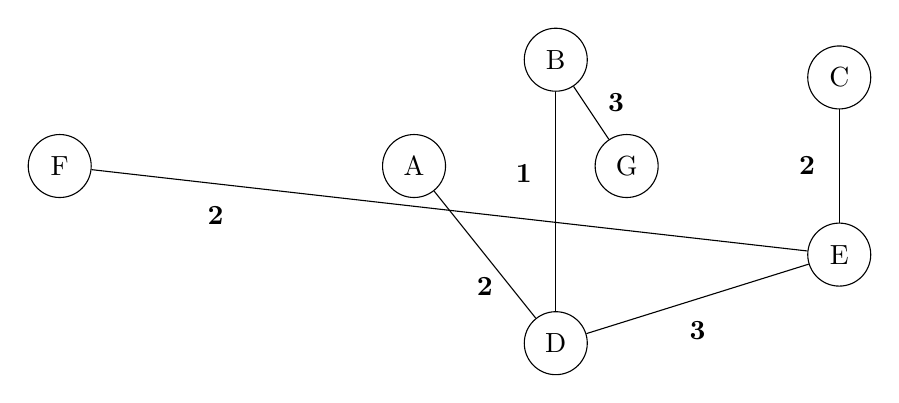
\begin{tikzpicture}[scale=0.9, every node/.style={circle, draw, minimum size=8mm}]
              \node (A) at (0,0) {A};
              \node (B) at (2,1.5) {B};
              \node (C) at (6,1.25) {C};
              \node (D) at (2,-2.5) {D};
              \node (E) at (6,-1.25) {E};
              \node (F) at (-5, 0) {F};
              \node (G) at (3, 0) {G};

              \draw (B) -- (D);
              \node[draw=none, left, font=\bfseries] at ($(B)!0.4!(D)$) {1};
              \draw (A) -- (D);
              \node[draw=none, below, font=\bfseries] at ($(A)!0.5!(D)$) {2};
              \draw (C) -- (E);
              \node[draw=none, left, font=\bfseries] at ($(C)!0.5!(E)$) {2};
              \draw (E) -- (F);
              \node[draw=none, below, font=\bfseries] at ($(E)!0.8!(F)$) {2};
              \draw (D) -- (E);
              \node[draw=none, below, font=\bfseries] at ($(D)!0.5!(E)$) {3};
              \draw (B) -- (G);
              \node[draw=none, right, font=\bfseries] at ($(B)!0.4!(G)$) {3};
            \end{tikzpicture}
            \]
            Peso total: \(1 + 2 + 2 + 2 + 3 + 3 = 13\).
            \newpage

            \item Aplicando el algoritmo de Prim desde el vértice \(A\):
            \begin{enumerate}
              \item Desde \(A\), la arista más corta es \(A \to D\) (peso 2). Agregamos \(D\).
              \item Desde \(D\), la arista más corta es \(D \to B\) (peso 1). Agregamos \(B\).
              \item Desde \(B\), la arista más corta es \(B \to G\) (peso 3). Agregamos \(G\).
              \item Desde \(G\), la arista más corta es \(G \to C\) (peso 4). Agregamos \(C\).
              \item Desde \(C\), la arista más corta es \(C \to E\) (peso 2). Agregamos \(E\).
              \item Desde \(E\), la arista más corta es \(E \to F\) (peso 2). Agregamos \(F\).
              \item No quedan más vértices por agregar.
            \end{enumerate}
            El árbol resultante es:
            \[
            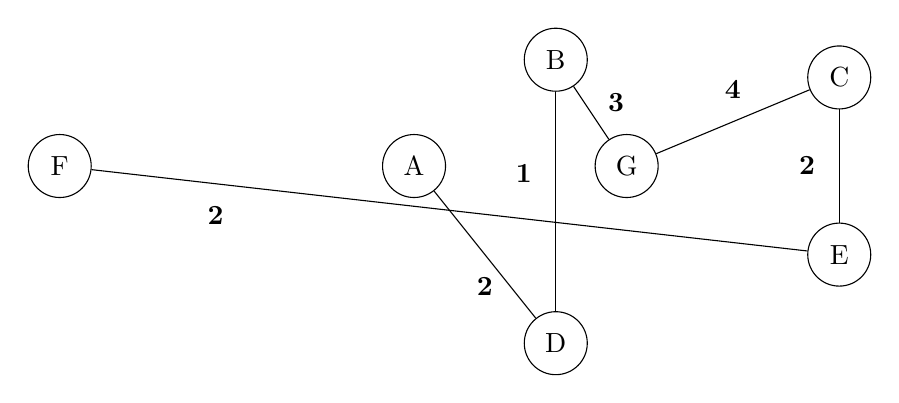
\begin{tikzpicture}[scale=0.9, every node/.style={circle, draw, minimum size=8mm}]
              \node (A) at (0,0) {A};
              \node (B) at (2,1.5) {B};
              \node (C) at (6,1.25) {C};
              \node (D) at (2,-2.5) {D};
              \node (E) at (6,-1.25) {E};
              \node (F) at (-5, 0) {F};
              \node (G) at (3, 0) {G};

              \draw (A) -- (D);
              \node[draw=none, below, font=\bfseries] at ($(A)!0.5!(D)$) {2};
              \draw (B) -- (D);
              \node[draw=none, left, font=\bfseries] at ($(B)!0.4!(D)$) {1};
              \draw (B) -- (G);
              \node[draw=none, right, font=\bfseries] at ($(B)!0.4!(G)$) {3};
              \draw (G) -- (C);
              \node[draw=none, above, font=\bfseries] at ($(G)!0.5!(C)$) {4};
              \draw (C) -- (E);
              \node[draw=none, left, font=\bfseries] at ($(C)!0.5!(E)$) {2};
              \draw (E) -- (F);
              \node[draw=none, below, font=\bfseries] at ($(E)!0.8!(F)$) {2};
            \end{tikzpicture}
            \]
            Peso total: \(2 + 1 + 3 + 4 + 2 + 2 = 14\).
            \item No, los MSTs no coinciden. Esto se debe a que el algoritmo de Kruskal y Prim pueden producir árboles de expansión mínima diferentes dependiendo del orden en que se procesan las aristas o los vértices, respectivamente.
          \end{enumerate}

        % RESPUESTA 6
        \item 
          \begin{enumerate}[label=\alph*)]
            \item Aplicando el algoritmo de Dijkstra desde \(A\):

            \vspace{0.5em}
            \textbf{Iteraciones:}
            \begin{enumerate}
              \item Inicializamos distancias: \(A\) (0), \(B\) (\(\infty\)), \(C\) (\(\infty\)), \(D\) (\(\infty\)), \(E\) (\(\infty\)), \(F\) (\(\infty\)), \(G\) (\(\infty\)).
              \item Visitamos \(A\) (0), actualizamos distancias: \\
                - Desde \(A\), actualizamos \(B\) (4), \(D\) (2), \(F\) (7).
              \item Visitamos \(D\) (2), actualizamos distancias: \\
                - Desde \(D\), actualizamos \(E\) (5), \(G\) (7).
              \item Visitamos \(B\) (4), actualizamos distancias: \\
                - Desde \(B\), actualizamos \(C\) (10).
              \item Visitamos \(C\) (10), no se actualizan distancias.
              \item Visitamos \(E\) (5), no se actualizan distancias.
              \item Visitamos \(F\) (7), no se actualizan distancias.
              \item Visitamos \(G\) (7), no se actualizan distancias.
            \end{enumerate}
            La tabla final de distancias es:
            \[
              \begin{array}{|c|c|}
                \hline
                \text{Vértice} & \text{Distancia desde A}\\
                \hline
                A & 0 \\
                B & 4 \\
                C & 10 \\
                D & 2 \\
                E & 5 \\
                F & 7 \\
                G & 7 \\
                \hline
              \end{array}
            \]
            \item El camino más corto de \(A\) a \(E\) es: \(A \to D \to E\) con una distancia total de 5.
          \end{enumerate}
      \end{enumerate}
\end{document}